\documentclass{llncs}

% UTF8 support
\usepackage[utf8x]{inputenc}
\usepackage{url}
\usepackage{graphicx}
\usepackage{float}

\usepackage{paralist}

\usepackage[draft]{fixme}
\usepackage{todonotes}

\graphicspath{{figs/}}
\newcommand{\eg}{{\textit{e.g.~}}}
\newcommand{\etal}{{\textit{et al.~}}}
\newcommand{\ie}{{\textit{i.e.~}}}

\begin{document}

\title{Simulation and HRI\\Recent Perspectives with the MORSE Simulator}

\author{
Séverin Lemaignan\inst{1} \and 
Marc Hanheide\inst{2} \and 
Michael Karg\inst{3} \and 
Harmish Khambhaita\inst{4} \and \\
Lars Kunze\inst{5} \and 
Florian Lier\inst{6} \and 
Ingo Lütkebohle\inst{7} \and 
Grégoire Milliez\inst{4}
}

\authorrunning{Séverin Lemaignan et al.}

\institute{CHILI Lab, EPFL, Lausanne, Switzerland
\and Centre for Autonomous Systems, University of Lincoln, United Kingdom
\and IAS, Technische Universität München, Germany
\and LAAS/CNRS, Université de Toulouse, France
\and Intelligent Robotics Lab, University of Birmingham, United Kingdom
\and CITEC, Universität Bielefeld, Germany
\and Machine Learning and Robotics Lab, Universität Stuttgart, Germany}



\maketitle

\begin{abstract}

Simulation in robotics is often a love-hate relationship: while simulators do
save us a lot of time and effort compared to regular deployment of complex
software architectures on complex hardware, simulators are also known to evade
many (if not most) of the real issues that robots need to manage when they enter
the real world.  Because humans are the paragon of dynamic, unpredictable,
complex, real world entities, simulation of human-robot interactions may look
condemn to fail, or, in the best case, to be mostly useless. This collective
article reports on five independent applications of the MORSE simulator in the
field of human-robot interaction: It appears that simulation is already useful,
if not essential, to successfully carry out research in the field of HRI, and
sometimes in scenarios we do not anticipate.

\end{abstract}

\section{Introduction}

The use of simulators for Human-Robot-Interaction (HRI) systems now encompasses 
a variety of use cases, from prototyping through evaluation
to anticipatory simulation at runtime. However, even more than robot software
in general, it suffers from an integration problem: Simulation in HRI requires
robot simulators in all their complexity \emph{plus} a means of representing 
and interacting with
human agents. Particularly the latter is currently very much in its infancy,
and restricted to special applications only.

We believe that an important stepping stone for wider use of simulation in HRI
is the availability of an integrated, easy-to-use framework that can encompass
all currently important use-cases, and that provides an integration interface 
for developers \emph{and} end-users of HRI simulation.  In particular, we feel
that it must be both easy to install and use, and offer \emph{domain 
abstractions} to facilitate development and integration.

This paper presents how recent work using the ``Modular OpenRobots Simulation
Engine'' (MORSE, figure~\ref{fig|morse-hri}~\cite{morse_simpar_2012}) simulator
attempts to address this challenge. In the following, we first review the variety of 
current use cases for simulation in HRI, then introduce MORSE with a focus on 
HRI-specific features, and finally demonstrate and discuss MORSE's versatility
through several case studies. 

The case studies also illustrate the collective nature
of this article: We report on contributions and experiences in human-robot interaction
simulation from five unrelated projects, conducted by different people in
different organizations, only sharing the MORSE simulator
as common simulation platform. 

%The sections~\ref{sc:assessment} to~\ref{sc:ci}
%present each of these projects, and try to highlight both the positive
%outcomes of deploying simulation environments for HRI, and the pitfalls and more
%fundamental issues that simulation of human-robot interaction still faces.

\subsection*{HRI and simulation}

\begin{figure}[t]
      \centering 
      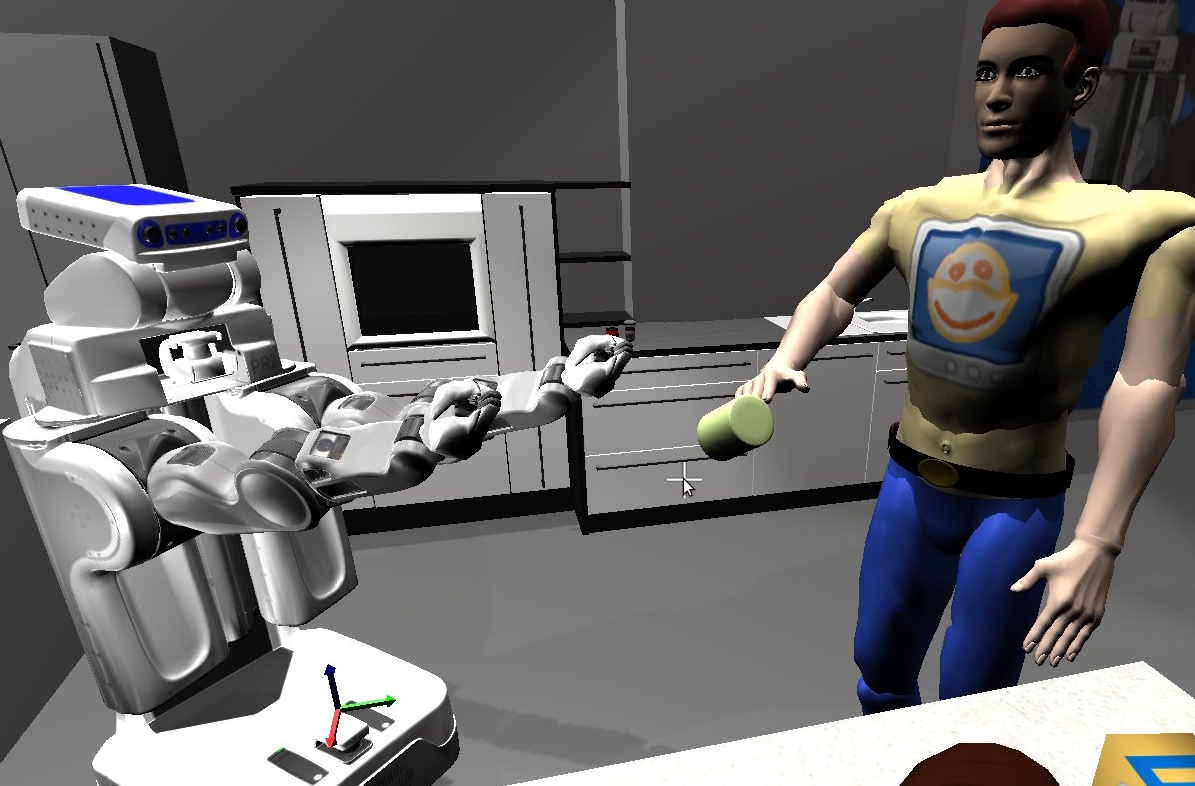
\includegraphics[width=0.7\linewidth]{morse_pr2.jpg}
      \caption{Simulation and HRI: A PR2 and a human avatar in MORSE.}
      \label{fig|morse-hri}
\end{figure}

When we mention simulators in the following, we refer to simulation engines with
support for physically simulating robot kinematics and dynamics, as well as
physical objects in the environment, and where the control and sensor interface
is close to or the same as it is on real robots. In this paper, we beside
only consider engines that support rendering, animation and control of human agents
suitable for HRI, and which have been actually used in this context (while many
engines could theoretically support this use case, few of them have actually
demonstrated it). For the interested reader, a broader overview of research in
robotic simulation is provided in~\cite{Ando2010}.

Besides MORSE, simulators with explicit support for controlling a human agent
include USARSim (Lewis~\etal\cite{lewis2007usarsim}), which is commonly used in
the field of rescue robotics and in dozens of HRI studies, and, to a
lesser extend, experiments with character animation have been developed in the
widely-used simulator Gazebo (Koenig and Howard~\cite{Koenig2004}).


%Note, however, that USARSim and MORSE are quite similar technically, in that
%both are based on an underlying game engine (the Unreal Tournament Development
%
%respectively), which has been extended with robot actuator and sensor models,
%and both support control through common middlewares. We prefer MORSE for its
%fully open source approach, and some other technical differences (see next
%section for more details), but we believe that due to the overwhelming
%similarities most, if not all, requirements and/or conclusions identified would
%also apply to work using USARSim.

All of these simulators are based on game engines (the Blender Game Engine,
Unreal Tournament Development Kit and Ogre3D, respectively). While their
built-in support for human models varies, all of these engines require the
developer to specify the agents' behavior in detail. In practice, this limits
human agent behaviors to relatively simple motions and interactions, and perhaps
not surprisingly, most HRI simulations so far are carried out either with
algorithmically-defined automatic human behaviors (typically, simulation of
crowds or
pedestrians) or in
\emph{tele-operation} settings, where only the robot and the environment, but
not the human agent, are actually simulated.

In contrast, current work on embodied virtual agents (EVA) usually provides
higher-level functionality, such as simulated emotion dynamics, behavior
generation based on action primitives, conversational dialogue systems, and up
to cognitive simulations. However, integrating these into a coherent system with
an acceptable interface remains challenging~\cite{gratch2002creating}. We do not
think that general-purpose simulators will acquire any of these functions soon.
However, they could be capable of integrating external components, for example,
by offering an interface for the Behavior Markup Language
popular in the EVA community, or by exposing a (lower-level)
H-Anim\footnote{\url{http://www.h-anim.org/}} interface. H-Anim is already
supported by Blender, MORSE's foundation.

That said, the use cases shown in the next sections hopefully demonstrate that
even with current limited functionalities, many relevant scenarios can already
be realized.

\subsection*{HRI and the MORSE simulator}

All five projects that are presented in this article rely on the MORSE as
simulation platform. In this section, we briefly go over the main MORSE features
and kindly suggest the interested readers to refer to~\cite{morse_simpar_2012}
or to the MORSE website\footnote{\url{http://morse-simulator.github.io}} for
details.

MORSE is a open-source tool developed for academic robotic research with
contributions from over 15 institutions worldwide. It is a domain independent
simulator where virtual robots can interact with a 3D environment, using sensors
and actuators that behave in the same way as their counterparts in the real
world. MORSE relies on the Blender \emph{Game Engine}, a real-time 3D runtime
integrated into the open-source Blender modeling toolkit, both for advanced 3D
(OpenGL shaders) and physics simulation (based on the {\sc Bullet} physics
engine\footnote{\url{http://www.bulletphysics.org}}). This allows for semi-realistic simulation of complex environments.
The MORSE components (sensors and actuators) exchange data with the robotics
software via middleware bindings (\emph{Software In The Loop} architecture).
Four robotics-related middlewares are currently supported, including ROS and YARP, as
well as a generic socket-based protocol. This design aims at providing a
seamless experience when switching back and forth between the simulator and the
physical robot. As expected for a versatile robotic simulator, standard
robotic platforms, actuators and sensors (more than 50 components) are
provided and enable fast creation of simulation scenarios. Additionally, custom
components can be added via Python (for the behaviors) and Blender (for the 3D
design).

%Two MORSE features stand out. First, MORSE has been primarily designed with a
%command-line interface, and only features a minimal (and fully optional)
%graphical user interface. This makes MORSE mainly targeted to an academic
%audience, where efficiency and lightness prevail.  Simulation scenes are
%actually short Python programs, thus well suited for sharing and versioning.
%This also eases the integration of the simulator into larger development
%workflows, and MORSE is successfully integrated into several continuous
%integration systems (Travis, Jenkins).

MORSE also introduces a concept of \emph{abstraction levels}: sensors and actuators
may expose several levels of abstraction, corresponding to different level of
realism. For instance, users may choose if the odometry sensor returns only a
curvilinear distance, a $dX, dY, dZ$ differential vector, or the absolute
position of the robot (integrated odometry). This allows users that are testing
low-level components to do so, while users working at higher abstraction
levels (typically in HRI) do not have to run full robotic software stacks (and
thus, benefit from a lighter environment) and can work in a more deterministic
environment. This feature can be finely controlled, on a per-component basis.

For HRI applications, MORSE provides a human avatar that can be fully controlled
(displacement, gaze, grasping of objects, interactions with the environment like
turning lights on, opening drawers, doors...) from a first-person-shooter perspective.
This enables the researcher to quickly setup and test human-robot interactions
with a tele-operated human model, hence with realistic human behaviors. As
presented in~\cite{lemaignan2012morse}, the human avatar can be controlled using
a Kinect-like device. The same avatar can also be programmatically controlled
by external scripts, like any robot in MORSE. With standard MORSE actuators like
the \emph{waypoint} actuator, the researcher can for instance pre-define paths
that the human avatar will follow in a simulated environment.

\section{HRI Simulation : Five Scenarios}

To illustrate how simulation can support research in HRI, we present in the next
sections five case-studies.  The first three scenarios, \emph{Situation
Assessment for HRI and Simulated Feedback}, \emph{An Expectations Framework for
Domestic Robot Assistants} and \emph{Preliminary Testing of Human-Aware
Navigation Planner} illustrate the typically use-case for simulation: rather
complex virtual environments are created where human presence plays a
central role, and HRI algorithms are tested in a convenient and repeatable way.
Note that, while we introduce here \emph{simulation-only} scenarios, they all
are test-cases of experiments that have been conducted on real robots:
simulation is used here to support real-world deployments.

The fourth scenario, \emph{Data Acquisition through Automatic Scene Generation}
shows how simulation is used as an alternative source of input to train robots to
behave in human environments, and the last scenario, \emph{Automated Execution
of Prototype HRI Experiments}, presents how the simulator can be used to provide
automatic testing of human-aware behaviors, fully integrated to the software
development workflow. Each of the presentations follow the same structure: we
first introduce the scenario, we then highlight how simulation has been leveraged
and its benefits, and we finally mention some of the shortcomings of the tool.

\subsection{Situation Assessment for HRI and Simulated Feedback}
\label{sc:assessment}

When studying human-robot interaction, understanding the environment in which
agents will interact is a key issue. In this first application, MORSE provides a
virtual environment that we use to harness situation assessment algorithms
(performed by a software called SPARK ~\cite{Warnier2012a}, for SPAtial
Reasoning and Knowledge) that also include human-centered \emph{perspective
taking}. The robot updates its knowledge in SPARK using its own position, human
position and objects seen through abstracted, symbolic cameras provided by MORSE
(so-called \emph{semantic} cameras). In this particular scenario
(figure~\ref{fig|spark}), the human is sitting in a couch and ask the robot to
bring specific objects that may be in another room.

\begin{figure}[t]
      \centering
      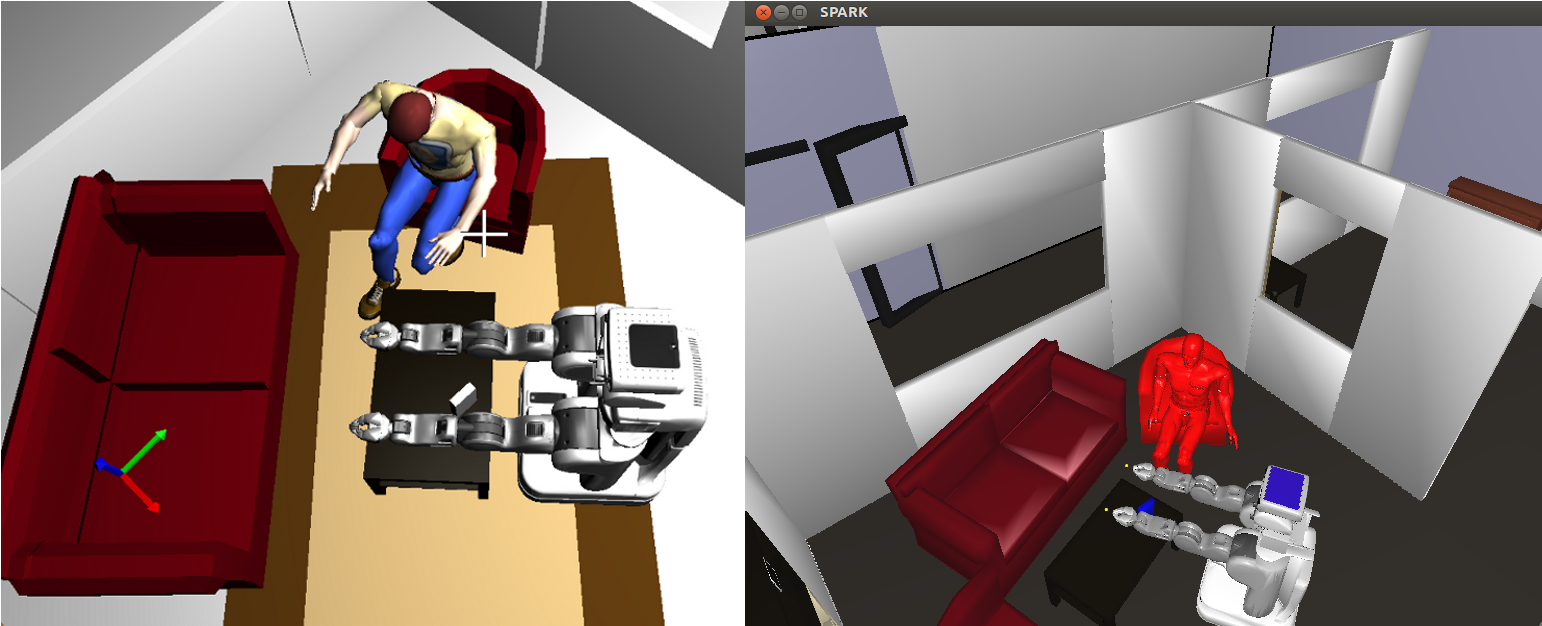
\includegraphics[width=0.7\linewidth]{morsespark.png}
      \caption{On the left side, the MORSE environment ; on the right side, the same
      environment, as perceived by the robot in the SPARK situation assessment
      module.}
      \label{fig|spark}
\end{figure}

\emph{Benefits of the simulation} The direct benefits of relying on MORSE for
the development of the situation assessment algorithms is the low-cost of
deployment (manual testing on physical systems is labour-intensive), as well as
the repeatability of the experimental conditions, important to assess the
algorithmic improvements.  Also, relying on MORSE effectively supports
collaboration between the partners involved in this project (MaRDi
project\footnote{\url{http://mardi.metz.supelec.fr}}): our partners are also
using MORSE simulation to test their software and collect data with the same
environment in their laboratory, where they focus on dialog processing. They can
train their dialog system using MORSE feedback to test the robot behaviors.

\emph{Specific limitations} MORSE currently only partially supports features
related to sound management (no simulation of microphones, no support for sound
propagation models), thus only providing an incomplete model of the environment.

\subsection{An Expectations Framework for Domestic Robot Assistants}
\label{sc:expectations}

In this scenario, an apartment is simulated in which a domestic service robot is
living together with a person (figure~\ref{fig|apartment}).  A PR2 robot is
controlled via ROS and the {\sc Cram} reactive plan language, which is used on
several other real robots. The robots' duty is to observe the person performing
different activities and detect unexpected situations based on the validation of
different types of expectations~\cite{Karg2013}.  The detection of such
unexpected behavior can help future domestic service robots to better assess
situations and adapt their actions to human behavior.

\emph{Benefits of the simulation} The use of the MORSE simulator enabled us to
set up a large testbed by reusing the real robot control layer via the ROS
middleware and easy-to-generate unpredictable human behaviors using the human
component of MORSE. Setting up of such an apartment in a real-world setting,
together with a suitable sensor setup and a reliable robot control, would not
only introduce huge costs but would also be a time-consuming task which can
distract researchers from their actual research focus. The use of the simulated
scenario enables us to gain many insights into the problem domain in a scenario
that would not been possible within our project, while the algorithms were
eventually validated on the real robot, inside a smaller real-world environment.

\begin{figure}[t]
      \centering
      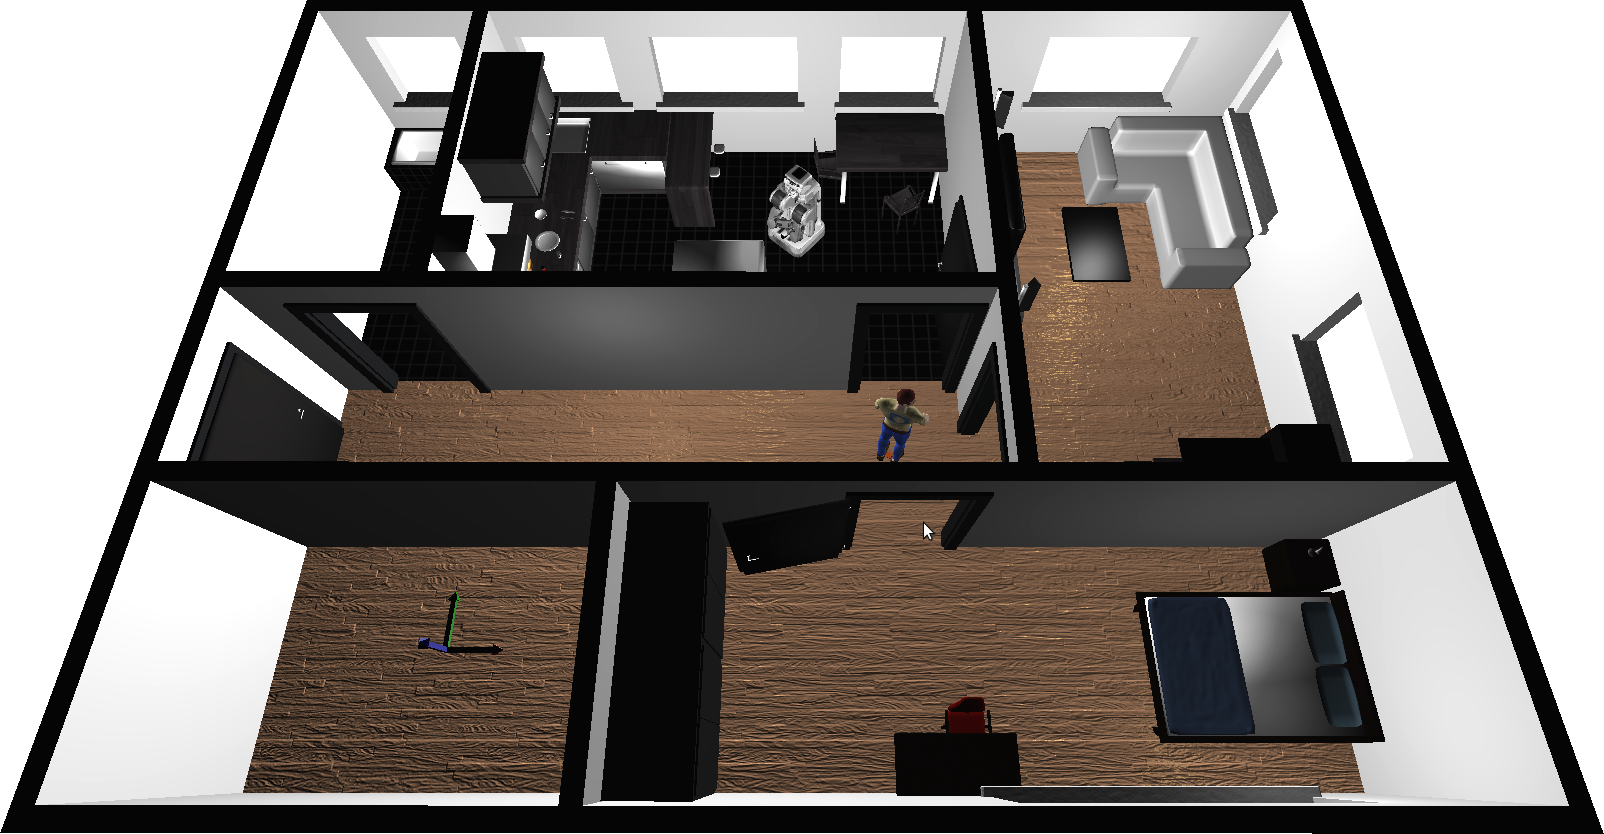
\includegraphics[width=0.7\linewidth]{morse_apartment.png}
      \caption{A simulated apartment with a domestic service robot and a person.}
      \label{fig|apartment}
\end{figure}

The human component of MORSE enabled us to test and validate our approach
dynamically in a variety of situations. Since it can be controlled in real-time
like in a 3D computer game while at the same time, a robot can be simulated by
state-of-the-art components, it is possible to generate a multitude of
situations on which the robot has to react. This greatly supported our project
to gain insights about our approach, detect weak points and make improvements.

\emph{Specific limitations} While the game-like control of the human avatar 
successfully enabled us to simulate simple actions like picking and placing objects, 
opening doors and using light switches, actions that require find-grained control 
of the arms and hands are not yet possible. For instance, when trying to set a table for 
diner, it is often not possible to accurately place objects like cutlery. Also, the human
avatar is currently restricted to using one arm which is unrealistic in activities 
like table setting, where humans often use both arms for pick and place actions.
 

\subsection{Preliminary Testing of Human-Aware Navigation Planner}
\label{sc:navigation}

To evaluate the improvements in the human-aware navigation planner developed at
LAAS we carried out a user study. An experiment was set up,
where a robot encounters a human crossing its path (at $90^{\circ }$ angle to
each other) while the robot is moving forward to its navigation goal. For
preliminary testing of the planning algorithm, our lab area was simulated in
MORSE. This simulated environment was extensively used
to review the algorithm before it was deployed on the PR2 robot to carry out
real-world experiments (whose results have been published
in~\cite{ThibaultKruse2014}).


\emph{Benefits of the simulation} Development of human-robot interaction
algorithms often require iterative process of prototyping, testing and
reviewing. Setting up and experiment and testing of robot navigation algorithms
especially for large environments involving humans is time consuming and is
subject to availability of lab resources while working in a shared lab between
different groups of researchers. Full support of the PR2 robot model among
others, availability of a human model, and a convenient way of setting up
experiment environment using Blender software were the most prominent features
for choosing MORSE as the simulation environment for these experiments. Since
MORSE already provides ROS bindings for the PR2 robot and human pose it requires
minimal effort to switch between real-world and simulated environments.

As a consortium member in the EU project
SPENCER\footnote{\url{http://www.spencer.eu}}, we plan to develop novel
algorithms for robot navigation in large populated environments, \eg airports.
In the future we plan to use MORSE to simulate such large environment with
multiple human models. This will certainly push the limits of simulation for HRI
and hopefully provide new benchmarks.

\emph{Specific limitations} All DoFs of the human posture in MORSE already have an
interface support for the {\sc pocolibs} and YARP middleware. A ROS interface
for the same would be a valuable addition, by publishing these DoFs
as coordinate frames using the typical {\tt tf} package. Moreover, an easier
way to attach camera to the human eyes would be appreciated. For HRI experiments
this will give a human perspective on the robot actions and its effects on the
environment.


\subsection{Data Acquisition through Automatic Scene Generation}
\label{sc:generation}

This fourth study proposes a different perspective on the role of simulation in
HRI: simulating credible human environments to train systems to appropriately
react to them: autonomous mobile robots that are to help and assist people in
care homes, households, and at other workplaces have to understand how human
activities affect the dynamics of objects in the environment. That is, robots
need to know, when, where and how people manipulate objects and how they arrange
and structure them in space. In the context of the STRANDS
project\footnote{\url{http://www.strands-project.eu}} we aim for robots that
understand the long-term, spatio-temporal relationships of objects and
activities of people. In the scenario described here, we looked in
particular at learning qualitative spatial relations of objects on office desks.
As an accurate classification and pose estimation of objects on real-world
office desks is still a challenging and difficult task for current robot
perception systems we acquired a data set of object arrangements using the MORSE
simulator. For this, we first bootstrapped an object statistics from manually
labeled images of real office desks, and secondly, automatically generated a set
of physically possible desktop scenes
(figure~\ref{fig:simulated-desktop-scenes}). Based on the generated data we
learned relational models of object arrangements on desks. The learnt models
enabled a robot to predict the position of an object given a landmark. We
employed these models to effectively guide a simulated and a real robot in
object search tasks and evaluated its performance~\cite{kunze14indirect}.

\emph{Benefits of the simulation} First, the automatic scene generation (made
easy by the use of Python to ``program'' the simulation scenes) and annotation
of object arrangements in simulation is useful for the acquisition of large
amounts of data over short periods of time. The generated data enabled us to
design, implement and to evaluate our methods for predicting object locations
before having a real-world data set in place. Secondly, the generation of object
arrangements can increase the variability of scenes in human-robot experiments
in general. Given the dynamics of objects in the real world it is important not
to oversimplify human-robot experiments in simulated environments but make them
as realistic as possible (in a controlled way). Finally, in future work, we plan
to use the generated desktop scenes in web-applications to crowdsource Natural
Language descriptions of object arrangements and commands for robots from
Internet users.

\emph{Specific limitations} A desirable feature would be that
objects are kept in a global or some domain specific object databases and that
they are modeled in a consistent way. This would ease the usage of different
types of objects and thereby allow users and researchers to focus on their
goals. Also the addition and/or removal of objects at run-time would be a nice
feature as a running MORSE instance could be used more flexible, for example,
as a robot's belief state.

\begin{figure}[t]
  \centering
  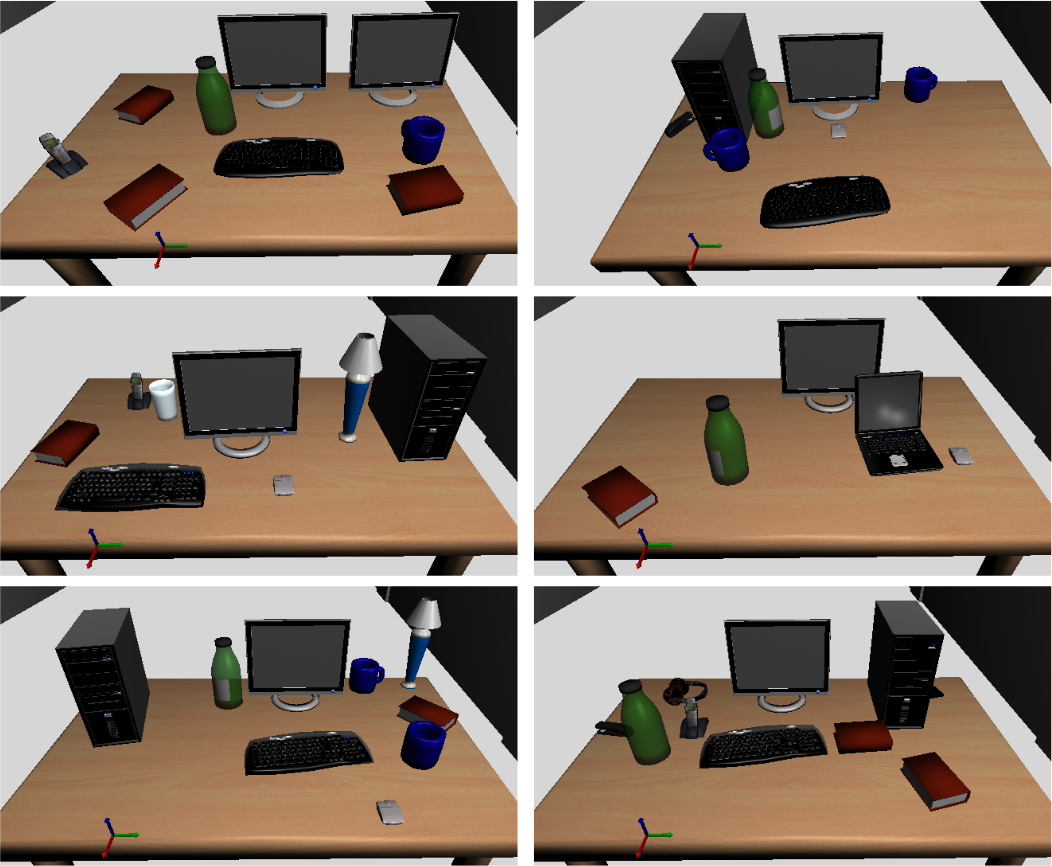
\includegraphics[width=.7\columnwidth]{figs/scenes.png}
  \caption{Automatically generated scenes of office desks.}
  \label{fig:simulated-desktop-scenes}
\end{figure}


\subsection{Automated Execution of Prototype HRI Experiments}
\label{sc:ci}

In human-robot interaction studies, robots often indicate behavioral variability
that may influence the experiment's final outcome.  However, manual testing on
physical systems is usually the only way to prevent this, but remains
labour-intensive. To tackle this issue, we introduced \emph{early automated
prototype testing}~\cite{2645922} that consists of: a simulation environment, a
software framework for automated bootstrapping of prototype systems, execution
verification of system components, automated result assessment of experiments
and a Continuous Integration (CI) server to centralize experiment execution. In
our setup we bootstrap and execute a simulated prototype system on a CI server
and assess the results in each run. In this particular scenario, a robot must
report the location of a virtual human in a domestic environment. Both the
robot and the human are moving in the scene and meet in front of a table.


The goal of this simulation setup is to incrementally decrease the level of
abstraction until a satisfactory/sufficient degree of ``realism'' to make an
assumption about real world behavior, is reached --- in an integrated and
continuous approach. In order to achieve this goal, we make use of two essential
MORSE features: \textit{a)} the human avatar that can be steered (set waypoints)
interactively via middleware and \textit{b)} a \emph{semantic} camera that
extracts the location of a specific entity in the simulation environment.  The
semantic camera is attached to the robot. If the human enters the robot's field
of view, the location is reported and sent via middleware. After each CI run,
the recorded movement trajectory of the human avatar is assessed (plotted) and
archived. We have explicitly chosen to simplify the extraction of the location
of the human to acquire a ground truth in the first iterations of the
simulation. Based on the ground truth, we are able to exchange diverse
components, \ie the semantic camera with a simulated laser scanner to build a
person hypothesis for instance, thus gradually develop, assess and implement
more complex scenarios. 

\emph{Benefits of the simulation} First of all, the interactive (remotely
controllable) human avatar is useful to include a dynamic, yet not too
realistic, human component in this setup, which currently is a rare feature in
the world of simulators. Secondly, the level of abstraction of different
sensors, \ie semantic camera versus virtual laser scanner enables us to
gradually raise the level of complexity/realism and test different algorithms
based on abstract and almost realistic sensor inputs.  Lastly, the chance to
deploy MORSE in a Continuous Integration environment, \ie automatically run
simulation scripts, generates an additional benefit.
 
\emph{Specific limitations} To be even more useful, simulators and thus MORSE, must
feature a realistic ``walking cycle'' for human components. This is especially
important if laser scans are used to build a person hypothesis. Additionally, the
human avatar should feature (remotely) triggered ``actions'', \eg grasping a 
predefined object, sit down on a chair/sofa or open a door. Lastly, audio support, 
\ie Text-to-Speech output for the human component would significantly increase
the usability to assess algorithms which rely on multimodal inputs.  

\section{Discussion: Towards Unification}

Looking at recent literature on simulation and HRI, several distinct approaches
seem to emerge. In Henry et al.~\cite{henry2010learning}, the simulator is used
for evaluating their approach to navigation in crowds, prior to real-world
evaluation. In contrast, Garrell et al.~\cite{garrell2010model} describe the
\emph{real world validation} of a pedestrian model, with the eventual goal of
using that model for simulation. Kidokoro et al.~\cite{kidokoro2013will} (in a
somehow similar way to Hoffmann and Breazeal~\cite{hoffman2010effects}) take a
different approach and use a simulator to compare different situations. They use
the simulator as a \emph{computation engine} for spatial computations (in this
case, human comfort in the different situations). Finally, Breazeal et
al.~\cite{breazeal2013crowdsourcing} represent yet another use case, with the use
of the simulation inside a game environment that allows humans to play the
various agents, generating easily captured data for later analysis.

While the five scenarios that we present here implement different use-cases,
they actually cover similar approaches, while relying on the same simulator:
study~\ref{sc:assessment} shows how MORSE can be thought as a computation
engine, \ref{sc:expectations} exploits the human agent in a computer game style,
\ref{sc:navigation} uses MORSE for assessing and tuning the performance of
algorithms, and scenario~\ref{sc:generation}, while somewhat unique, still share
similarities with Garrell et al., in that a model for object positions is
trained on real-world data. Finally, the use-case presented in~\ref{sc:ci}
proposes a different approach, with a focus on continuous testing, and can
arguably be seen as the natural progression of using simulators for evaluation,
extended here to cover HRI scenarios.

From this perspective, one may consider that the experiments recently conducted
in the MORSE community around the simulation of HRI applications constitute the
first steps towards building an unifying platform for HRI simulation, with two
additional features: its \emph{programmability} (simulation scenarios are Python
scripts) and its concept of \emph{abstraction levels} that provides an effective
way to focus simulation on a particular problem by hiding irrelevant simulation
artifacts.

These diverse use-cases support the idea that simulation is not only actually
useful as a support tool for development of human-robot applications, but also
\emph{enables} new research techniques in HRI. \emph{Continuous Integration}
illustrates this point: while HRI experiments are considered as notoriously
difficult to deploy, test and repeat, we show here how a simulator may enable
automated testing of more and more complex scenarios, including long-term
interaction.

Several issues are also raised and must be clearly stated. In its current state,
the MORSE simulator provides only an incomplete model of the environment.
Sounds/speech models are incomplete, and human models do not yet provide good
enough accuracy, both at the level of the user interface (some actions can not
be done with the interactive avatar), and at the simulation level (poor/missing
walking cycles for instance). Finally, the overall convenience of MORSE for HRI
could be improved, for instance by providing more assets (furnitures, objects)
related to human environments. These issues, that are mostly technical and could
be addressed at the software level, show that simulators dedicated to HRI
application still need to mature. In that regard, the next section presents some
of the directions that are currently researched.

\subsection*{The next steps}

Several noteworthy developments related to HRI are currently shaping up in the
MORSE community. We outline below some of them, that suggest new applications
that we believe are relevant to HRI research.

A first line of investigation relates to the procedural generation of a variety
of realistic human models. {\sc MakeHuman} is such an open-source tool that
generates anatomically, kinetically and visually realistic human models. This
software has a tight integration with Blender, and MORSE is soon to provide as
well seamless integration with {\sc MakeHuman} models. This will bring a wide
range of characters to feed the simulations, and extend testing environments
with gender/size/age/skin color variances.

Besides being able to control a human avatar in simulation programmatically and
deterministically, the possibility to automatically generate believable and
realistic crowd behaviors is being explored. In this context, the objective is
to adopt in MORSE technologies previously developed for computer games to generate
trajectories that control the MORSE avatars. Based on the idea of \emph{social
forces}, the work of~\cite{Szymanezyk2012crowd} is to be
adapted to provide believable and realistic movement of several humans within
MORSE. This
implementation would provide a more realistic and dynamic environment to study
human-robot spatial interaction and to provide a testbed for human-aware motion
planning, to give two exemplary use cases.

Another line of investigation looks at \emph{embedding} the researcher into the
robotic simulation. The purpose of such efforts is to provide a life-like
immersive simulation environment that would allow at the same time ecologically
valid human behaviors and repeatable, lightweight interaction settings.
In~\cite{lemaignan2012morse}, we presented how a human agent could interact with
a virtual robot through a deictic interface based on a Kinect. Two distinct
projects are currently looking into extending this approach, one (at Bielefeld
University) aiming at integrating emerging Virtual Reality devices (like Occulus
Rift) with MORSE, the other one (MarDI project) developing a virtual reality
cave, that include 360° projections and spatialized sound.

Also often suggested, the \emph{on-line} deployment of HRI simulations could
efficiently support large scale HRI studies. The simulator and specific
interaction scenarios would be embedded in a dedicated webpage and users would
control a human avatar from their webbrowsers. This would potentially enable
collection of large behavioral datasets. While MORSE development in that
direction has yet to start, Breazeal et al. presented an initial attempt in that
direction in~\cite{breazeal2013crowdsourcing} and the Gazebo simulator features
a limited WebGL client that act as a proof-of-concept of on-line robotic
simulation.

%Faster-than-realtime simulation, a recent feature of MORSE (currently at testing
%stage), is a last development that can have significant applications for
%HRI\fixme{finish that}

\subsection*{Conclusion}

These examples and ideas hopefully give a picture of the lively landscape of the
``Simulation for HRI'' community, that has built itself around the MORSE
simulator.  In the introduction, we mentioned how simulation in HRI had to
address in parallel constraints stemming from \emph{robotic simulation} and
\emph{virtual agent simulation}, while remaining a lightweight, easy-to-use
tool. We are certainly not yet there, much remains to be imagined, refined and
achieved.  Yet MORSE is already deployed in several institutions as a platform
that efficiently supports research in human-robot interaction. As an open-source
project, we strive for new use-cases and ideas, and warmly welcome researchers
that would like to join the effort.


\section*{Acknowledgment}

This research has received funding from the European
Union (FP7/2007-2013) under grant agreements
FP7-600623 (STRANDS) and FP7-600877 (SPENCER).

\bibliographystyle{abbrv}
\bibliography{main}

\end{document}
